\documentclass[tikz,border=10pt]{standalone}
\usepackage{tikz}

\begin{document}
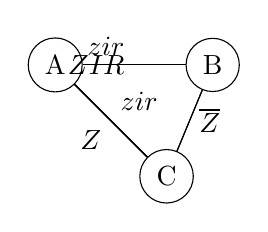
\begin{tikzpicture}[node distance=2cm]
    % Define nodes
    \node (A) [circle,draw] {A};
    \node (B) [circle,draw,right of=A] {B};
    \node (C) [circle,draw,below right of=A] {C};

    % Draw edges
    \draw (A) -- (B);
    \draw (A) -- (C);
    \draw (B) -- (C);
    \draw (A) -- (B);
    \draw (A) -- (C);

    % Label zir, Z, overline Z, and ZIR (assuming these are labels for edges)
    \path (A) edge node[above left] {$\operatorname{zir}$} (B);
    \path (A) edge node[below left] {$\operatorname{Z}$} (C);
    \path (B) edge node[right] {$\overline{\operatorname{Z}}$} (C);
    \path (A) edge node[left] {$\operatorname{ZIR}$} (B);
    \path (A) edge node[above right] {$\operatorname{zir}$} (C);
\end{tikzpicture}
\end{document}